%\documentclass[11pt,handout]{beamer}
%\documentclass{beamer}
\usepackage[ngerman]{babel}
\usepackage[utf8]{inputenc}
\usepackage{amsmath}
\usepackage{amssymb}
\usepackage{listings} 
\usepackage{stmaryrd}
\lstset{language=Python, tabsize=4, showstringspaces=false,basicstyle=\footnotesize,mathescape=true} 
\lstset{literate=%
  {Ö}{{\"O}}1
  {Ä}{{\"A}}1
  {Ü}{{\"U}}1
  {ß}{{\ss}}1
  {ü}{{\"u}}1
  {ä}{{\"a}}1
  {ö}{{\"o}}1
} 
\usepackage{mathtools}
\usepackage{ulem}
\usepackage{tikz}

\usetheme{Boadilla}
\mode<presentation>{
\useoutertheme[subsection=false]{miniframes}
\useinnertheme{rectangles}
%\usecolortheme{crane}
}
\parskip 10pt



\begin{document}
\title{Informatik}   
\author{Graphen 3} 
\date{}
\frame{\titlepage} 

%---
\begin{frame}[fragile]

Die Länge eines Pfades in einem ungewichteten Graphen ist die Anzahl seiner Kanten. Die Entfernung zweier Knoten 
in einem ungewichteten Graphen ist die Länge des kürzesten Pfades zwischen ihnen.

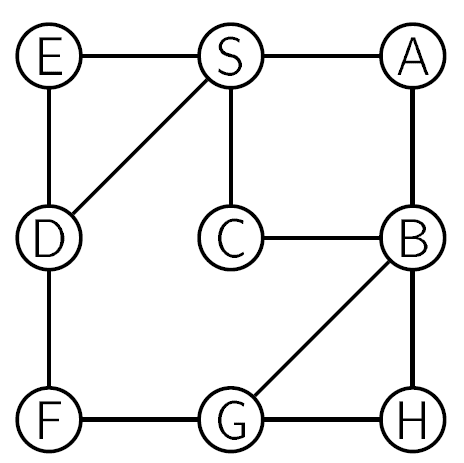
\includegraphics[height=4cm]{bild41.png}

Die Entfernung zwischen S und H ist \pause 3.
\end{frame}

\begin{frame}[fragile]

Die \textbf{Breitensuche} (breadth first search, bfs) traversiert den Graphen in Schichten nach der Entfernung zum Ausgangsknoten.
Zu jedem Knoten merkt man sich seinen Vorgänger (prev), dadurch entsteht ein shortest-path Baum.
(Ein Baum ist ein zusammenhängender Graph, der keine Kreise enthält). Daraus lässt sich der kürzeste
Weg vom Ausgangsknoten zu jedem anderen Knoten rekonstruieren.



\end{frame}

\begin{frame}[fragile]
Der shortest-path Baum der Breitensuche:

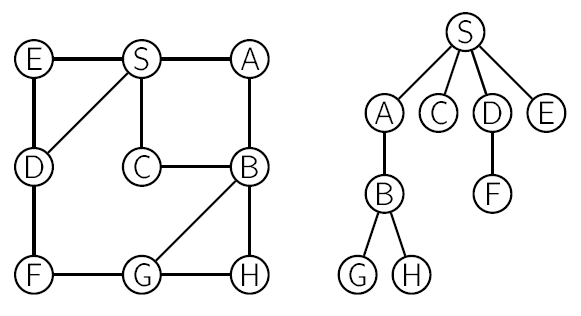
\includegraphics[width=9cm]{bild42.png}

\end{frame}

\begin{frame}[fragile]
Breitensuche mit Ausgangsknoten s:
\begin{lstlisting} 
Für jeden Knoten u in G: 
      dist(u) = unendlich 
      prev(u) = None

Füge s in eine Schlange Q ein 
dist(s) = 0

Solange Q nicht leer:
	hole Knoten u aus der Schlange
      für alle Nachbarn v von u:
           Falls dist(v) unendlich:
                 Füge v in die Schlange Q ein
                 dist(v) = dist(u) + 1
                 prev(v) = u
\end{lstlisting}
\end{frame}

\begin{frame}[fragile]
\begin{lstlisting} [basicstyle=\scriptsize]
def reconstructPath(s,u,prev):
    temp = []
    while u != s:
        temp.append(u)
        u = prev[u]
    temp.append(s)
    temp.reverse()
    return temp

from collections import deque       
inf = float('inf')
dist = {v:inf for v in G}
prev = {v:None for v in G}

s = 'S'         # Startknoten
dist[s] = 0     
Q = deque([s])       
while Q:
    u = Q.popleft()
    for v in G[u]:
        if dist[v] == inf:
            Q.append(v)
            dist[v] = dist[u]+1
            prev[v] = u
print(*(reconstructPath('S','H',prev))

\end{lstlisting}
\end{frame}

\begin{frame}[fragile]
Der Algorithmus von Dijkstra findet  in einem gerichteten, mit nichtnegativen Kosten gewichteten
Graphen die kürzesten Wege von einem Startknoten zu allen anderen Knoten.
\textit{(single source shortest paths)} \pause

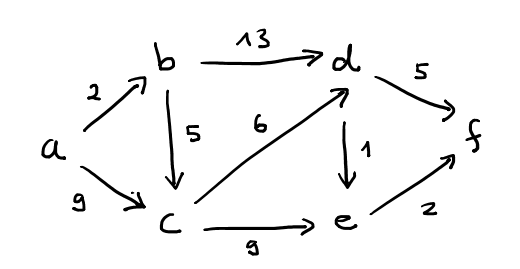
\includegraphics[width=10cm]{bild43.png}
\end{frame}

\begin{frame}[fragile]
Algorithmus von Dijkstra mit Startknoten s:
\begin{lstlisting}[basicstyle=\scriptsize]
Setze dist des Startknotens s vorläufig auf 0,
    alle anderen vorläufig auf unendlich. 
Setze prev aller Knoten auf None
Solange es noch vorläufige Knoten gibt
    setze dist des billigsten vorläufigen Knoten auf endgültig
    Für jeden Nachbarn v von u:   
        # Relaxiere Kante (u,v) 
        dist(v) = min(dist(v),dist(u) + Kosten von u nach v) 
        prev(v) = letzter Knoten auf dem Weg zu den minimalen Kosten
\end{lstlisting} \pause

Während des Algorithmus müssen wir uns aus den vorläufig markierten Knoten laufend einen billigsten suchen. \pause
Dazu nutzen wir einen Heap. \pause

Die Laufzeit hängt ab vom Aufwand der Operationen  zur Entnahme der Knoten aus dem Heap und zur Anpassung
der Distanzwerte. Bei einen Fibonacci-Heap ist beides $O(1)$ und der Aufwand also $O(\left|V\right|+\left|E\right|)$.
Aufwand bei einem Min-Heap: $O((\left|V\right|+\left|E\right|)\cdot\log\left|V\right|)$.
\end{frame}

\begin{frame}[fragile]
\begin{lstlisting}[basicstyle=\scriptsize]
# Algorithmus von Dijkstra
inf = float('inf')
dist = {v:inf for v in G}
prev = {v:None for v in G}

s = 'a'         # startknoten
dist[s] = 0
visited = set()

heap = [(dist[v],v) for v in G]
heapify(heap)
 
while heap:
    _, u = heappop(heap)
    if u in visited: continue
    visited.add(u)
    for v in G[u]:
        if dist[v] > dist[u] + G[u][v]:  # Relaxieren 
            dist[v] = dist[u] + G[u][v]  # der 
            prev[v] = u                  # Kante (u,v)
            heappush(heap,(dist[v],v))
\end{lstlisting}

\end{frame}

\begin{frame}[fragile]
Der Algorithmus von \textbf{Bellman-Ford} kann auch mit negativen Kantengewichten umgehen, vorausgesetzt
es gibt keine Kreise mit negativem Gewicht.

\begin{lstlisting}[basicstyle=\scriptsize]
Setze dist des Startknotens auf 0,
    alle anderen auf unendlich. 
Setze prev aller Knoten auf None
Solange sich was ändert:    # höchstens $\left|V\right| - 1$ mal
	Fur alle Kanten (u,v):
            Relaxiere(u,v)   # d.h. ggf. Kosten von v via u-v verbessern
\end{lstlisting} \pause

Die Kante (u,v) relaxieren 
Laufzeit: $O(\left|V\right|\cdot\left|E\right|)$.

\end{frame}

\begin{frame}[fragile]
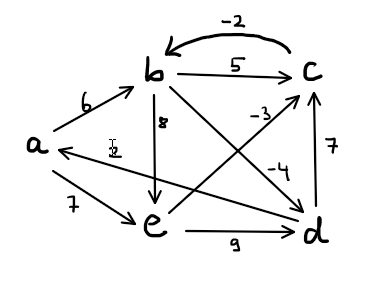
\includegraphics[width=6cm]{bellman_04.png} $\pause$

\begin{lstlisting}[basicstyle=\scriptsize]
0 :  a:0 b:inf c:inf d:inf e:inf
1 :  a:0 b:6 c:4 d:2 e:7
2 :  a:0 b:2 c:4 d:2 e:7
3 :  a:0 b:2 c:4 d:-2 e:7
4 :  a:0 b:2 c:4 d:-2 e:7
\end{lstlisting} \pause
\end{frame}

\begin{frame}[fragile]
\begin{lstlisting}[basicstyle=\scriptsize]

inf = float('inf')
dist = {v:inf for v in G}
prev = {v:None for v in G}

s = 'a'         # startknoten
dist[s] = 0

changed = True
while changed:
    changed = False
    for u in G:    
        for v in G[u]:
            if dist[v] > dist[u] + G[u][v]:
                dist[v] = dist[u] + G[u][v]
                prev[v] = u
                changed = True

\end{lstlisting}
\end{frame}

\begin{frame}[fragile]
Minimale Spannbäume (minimal spanning tree, MST)

1. Ein Teilgraph H eines ungerichteten Graphen G heisst Spannbaum von G, wenn H ein Baum auf den Knoten von
G ist. 

2. Ein Spannbaum S eines gewichteten, ungerichteten Graphen heisst minimaler Spannbaum, wenn S minimales Gewicht unter allen Spannbäumen von G besitzt.

\end{frame}
\begin{frame}[fragile]

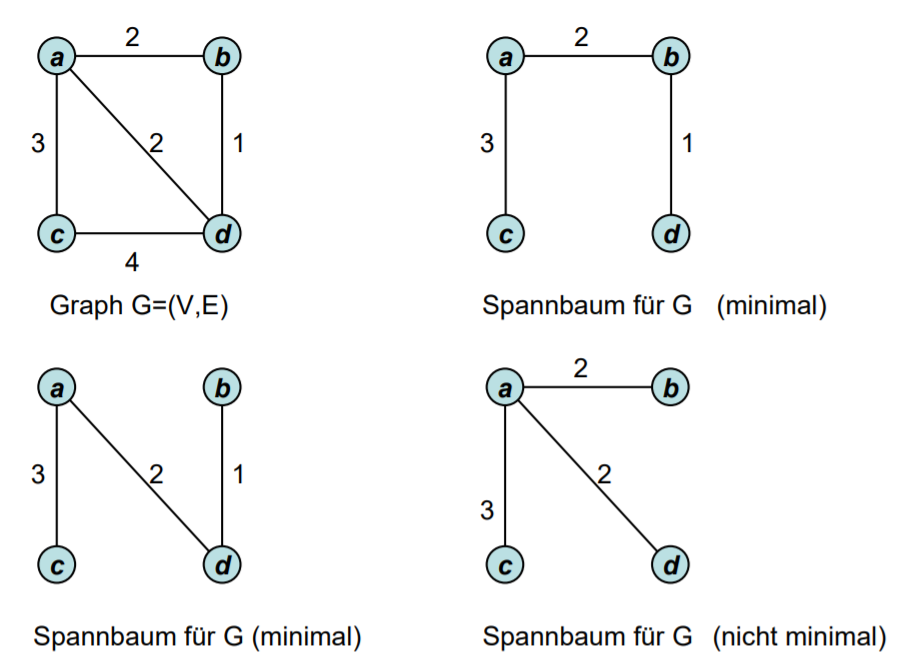
\includegraphics[width=11cm]{bild46.png}

\end{frame}


\begin{frame}[fragile]
Anwendung: Man möchte kostengünstig Computer vernetzen:

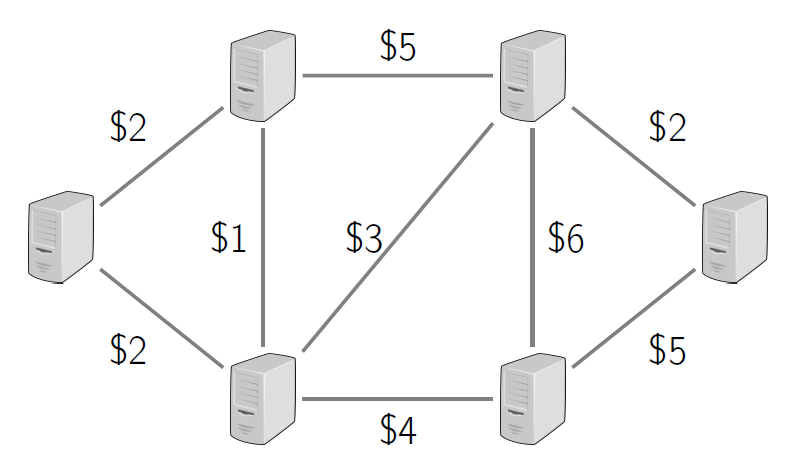
\includegraphics[width=11cm]{bild47.png}

\end{frame}

\begin{frame}[fragile]

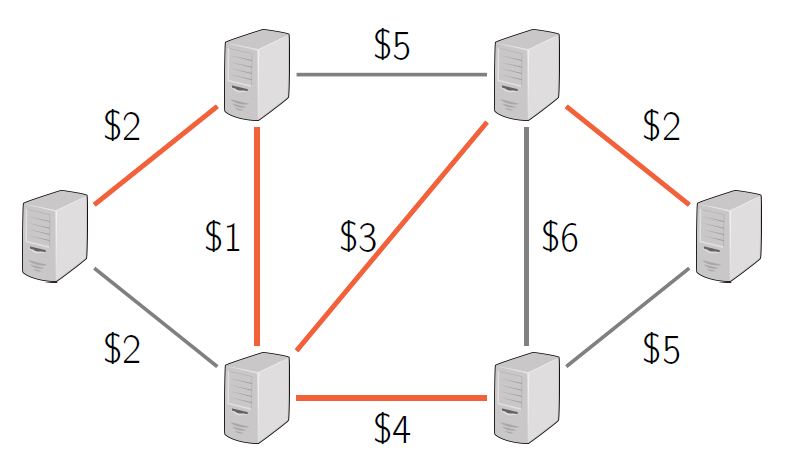
\includegraphics[width=11cm]{bild48.png}

\end{frame}

\begin{frame}[fragile]
Man möchte Orte mit möglichst kurzen Straßen verbinden.

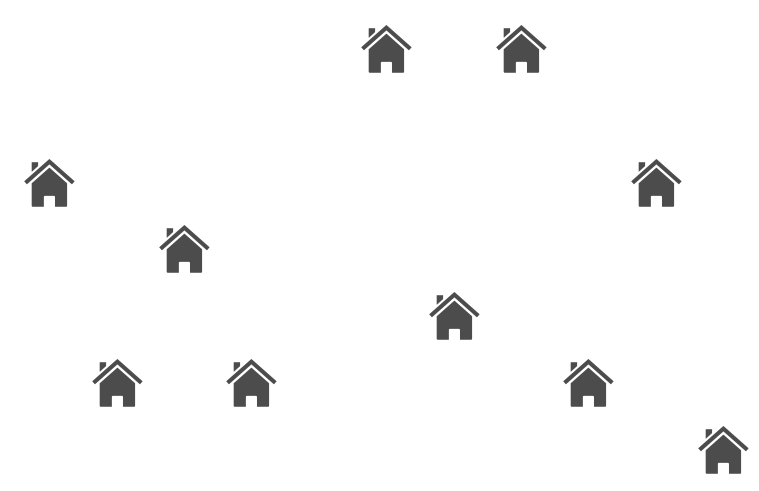
\includegraphics[width=11cm]{bild49.png}

en
\end{frame}

\begin{frame}[fragile]
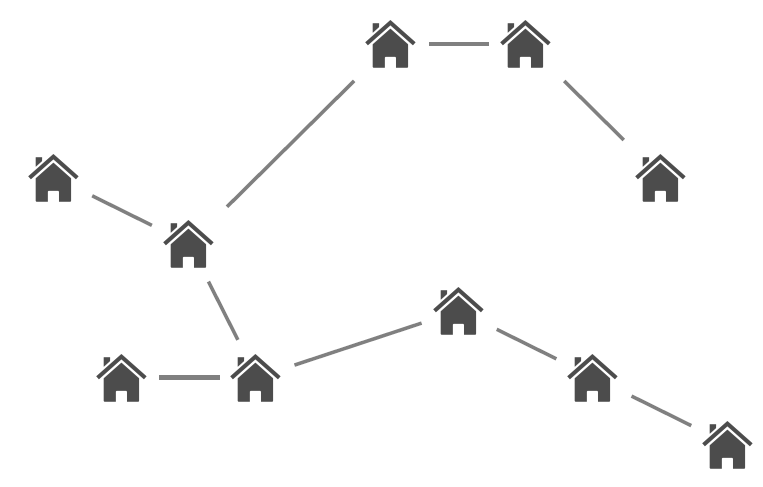
\includegraphics[width=11cm]{bild50.png}
\end{frame}

\begin{frame}[fragile]
Eigenschaften von Bäumen:

\begin{itemize}
\item Ein Baum ist ein zusammenhängender, ungerichteter Graph, der keine Kreise enhält.

\item Ein Baum mit $n$ Knoten hat $n-1$ Kanten.

\item Jeder zusammenhängende, ungerichtete Graph mit $\left|V\right| = \left|E\right| - 1$ ist ein Baum.

\item Ein ungerichteter Graph ist genau dann ein Baum, wenn es zwischen je zwei Knoten einen eindeutigen Pfad gibt.

\end{itemize}
\end{frame}

\begin{frame}[fragile]
Algorithmus von Kruskal: Füge immer wieder die leichteste Kante hinzu, vorausgesetzt es entsteht kein Kreis.

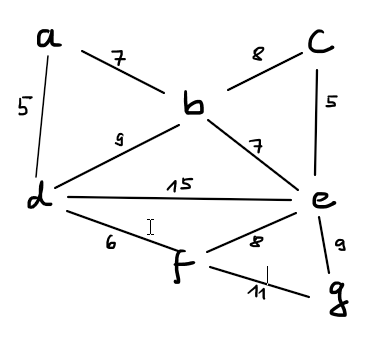
\includegraphics[width=5cm]{kruskal_03.png} $\pause$
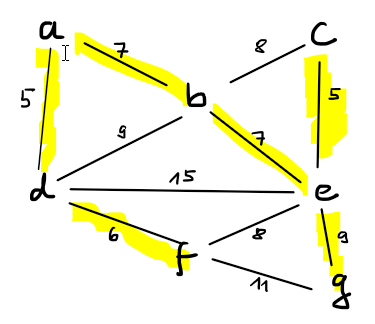
\includegraphics[width=5cm]{kruskal_03_mst.png}  

a-d (5), c-e (5), d-f (6), a-b (7), b-e (7), e-g (9), Gesamtkosten:  39

\end{frame}

\begin{frame}[fragile]
Um zu verhindern, dass ein Kreis entsteht, wird jedem Knoten ein Repräsentant ('Chef') zugeordnet.
Eine Kante wird nur in den MST aufgenommen, wenn die beteilgten Knoten nicht denselben Chef haben.
 $\pause$
\begin{minipage}[c]{6cm}
\begin{lstlisting}[basicstyle=\scriptsize]
a-d: 5   Chef von a wird d
c-e: 5   Chef von c wird e
d-f: 6   Chef von d wird f
a-b: 7   Chef von f wird b
b-e: 7   Chef von b wird e
e-g: 9   Chef von e wird g
\end{lstlisting}
\end{minipage}
\begin{minipage}[c]{5cm}
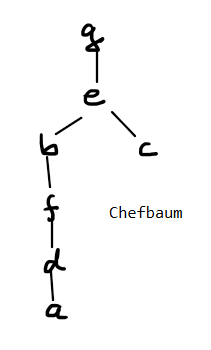
\includegraphics[width=3cm]{kruskal_03_chefbaum.png}
\end{minipage}
\end{frame}

\begin{frame}[fragile]
Um lange Pfade im Chefbaum zu verhindern, wird der Algorithmus mit \texttt{union by rank} und \texttt{path compression} optimiert.

 Wird der Chef von a gesucht,  dann werden alle Zwischenknoten auf dem Weg zum Chef direkt mit
diesem verbunden. Jeder Knoten erhält einen Rang. Bei der Neuzuweisung eines
Chefs wird der Knoten mit dem höheren Rang Chef. Bei Gleichheit wird einer gewählt, dessen Rang
dann erhöht wird.

\end{frame}
\begin{frame}[fragile]
\begin{lstlisting}[basicstyle=\scriptsize]
a-d: 5   Rang a gleich Rang d : Chef von a wird d
Rang von d wird 1
c-e: 5   Rang c gleich Rang e : Chef von c wird e
Rang von e wird 1
d-f: 6   Rang d größer Rang f : Chef von f wird d
a-b: 7   Rang d größer Rang b : Chef von b wird d
b-e: 7   Rang d gleich Rang e : Chef von d wird e
Rang von e wird 2
Kompression: Chef von b wird e
Kompression: Chef von f wird e
e-g: 9   Rang e größer Rang g : Chef von g wird e
\end{lstlisting}

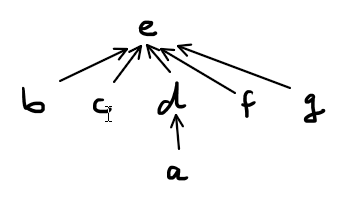
\includegraphics[width=5cm]{kruskal_03_opt_chefbaum.png}
\end{frame}
\begin{frame}[fragile]
Algorithmus von Prim: gehe von einem Knoten aus und füge immer wieder einen neuen Knoten entlang der leichtesten Kante hinzu.

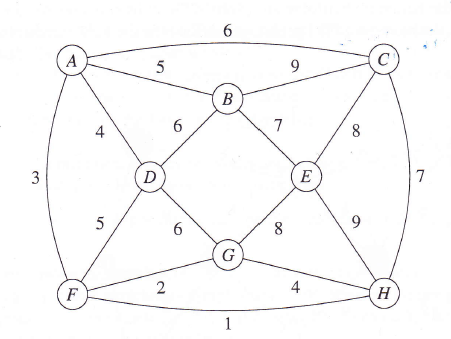
\includegraphics[width=8cm]{b7.png}

\end{frame}
 \end{document}